% Run 
% xelatex "\def\ishandout{1} % Run 
% xelatex "\def\ishandout{1} % Run 
% xelatex "\def\ishandout{1} % Run 
% xelatex "\def\ishandout{1} \input{main.tex}"
% to disable transition

\ifdefined\ishandout
  \documentclass[handout]{beamer}
\else
  \documentclass[]{beamer}
\fi

% Themes
\usetheme{default}

% Setup
\setbeamercovered{highly dynamic}
\newcounter{saveenumi}% save counter on enumerate across frames
\newcommand{\seti}{\setcounter{saveenumi}{\value{enumi}}}
\newcommand{\conti}{\setcounter{enumi}{\value{saveenumi}}}
\resetcounteronoverlays{saveenumi}

% Dependencies
\usepackage{fontspec} % use XeLaTeX
\usepackage[]{polyglossia}
\setdefaultlanguage{brazil}
\setmainlanguage{brazil}
% \usepackage{lcg} % Generate random numbers
\usepackage{hyperref}
\hypersetup{colorlinks=true,linkcolor=blue,anchorcolor=blue,urlcolor=blue}
\usepackage{pgf,tikz} % Draw figures
\usetikzlibrary{arrows,automata,calc,chains,circuits,graphs,positioning,shapes.gates.logic.US,shapes,trees}
\usepackage{circuitikz}
%\usepackage{pgfgantt}
  % \usepackage{pgfplots}
  % \usegdlibrary{trees}
  \usepackage{listings}
  \lstset{language=C,inputencoding=utf8,basicstyle=\footnotesize, 
    flexiblecolumns=true, numbers=left, numberstyle=\tiny\color{gray}, 
    commentstyle=\scriptsize\color{black!50},mathescape}
  \usepackage{pdftexcmds} % \pdf@strcmp \pdf@filemoddate
  \usepackage{ifthen} % \ifthenelse
 
  % FONTS
  \font\fiverm=cmr5
  \font\ninerm=cmr9

  % Definitions
  \author{Adriano J. Holanda}%\\{\scriptsize \url{http://holanda.xyz}}}
  \def\array{vetor}
  \def\bigO#1{\mathcal{O}(#1)}
  \def\bug#1{{\it bug#1\/}}
  % C letter
  \font\ninerm=cmr9
  \let\mc=\ninerm
  \def\CEE{{\mc C\spacefactor1000}}

  \def\boxset{
    \tikzset{box/.style={rectangle,minimum width=.5cm,draw},
      index/.style={minimum width=.5cm}}
  }

  % only title frames
  \def\onlytitleframe#1{\author{}\date{}\title{#1}\maketitle}

  % THEOREM
  % \newtheorem{teorema}[theorem]{Teorema}

  \newcommand{\executeiffilenewer}[3]{%
    \ifnum\pdf@strcmp{\pdf@filemoddate{#1}}%
    {\pdf@filemoddate{#2}}>0%
    {\immediate\write18{#3}}\fi%
  }
  % includesvg[includegraphics args]{file} command (linux-version)
  \newcommand{\includesvg}[2][]{%
    \executeiffilenewer{#2.svg}{#2.pdf}{%
      /usr/bin/inkscape -z -C --file="#2.svg" --export-pdf="#2.pdf" > /tmp/#2.log}%
    \ifthenelse{\equal{#1}{}}{%
      \includegraphics{#2}}{%
      \includegraphics[#1]{#2}}%
  }

\def\lecturetitle#1#2{\title{{\large\bf#1}\\{\small [#2]}}}

\def\transitionslide#1{\frame{\author{}\title{\LARGE#1}\date{}\maketitle}}

  \def\shcmd#1{
    \begingroup
    \bigskip\color{gray}
    {\tt \$~#1}
    \bigskip
    \endgroup
  }

  \def\fonte#1{\begingroup\tiny\tt\color{gray} Fonte:~#1\endgroup}

\usecolortheme{beaver}
\usefonttheme{serif}

\usepackage{inconsolata}

\lstset{
    language=java,
    basicstyle=\ttfamily\small,
    numberstyle=\footnotesize,
    numbers=left,
    backgroundcolor=\color{gray!10},
    frame=single,
    tabsize=2,
    rulecolor=\color{black!30},
    escapeinside={\%*}{*)},
    breaklines=true,
    framextopmargin=2pt,
    framexbottommargin=2pt,
    inputencoding=utf8,
    extendedchars=true,
    literate={á}{{\'a}}1 {ã}{{\~a}}1 {é}{{\'e}}1,
}

\def\course{Auditoria e Segurança de Sistemas}

% Table of Contents
\AtBeginSection[]
{
  \begin{frame}
    \frametitle{Table of Contents}
    \tableofcontents[currentsection]
  \end{frame}
}

\begin{document}
% \date{11/8/2021}\input intro

%\date{18/8/2021} \input dev

%\date{25/8/2021} auditoria em arquivos do Windows (Google Slides)

%\date{1/9/2021}\input net

%\date{8/9/2021}\input malware

%\date{22/9/2021}\input vpn
%\date{22/9/2021}\input proxy

%\date{06/10/2021}\input wireless

\lstset{language=java,basicstyle=\scriptsize,keywordstyle=\color{green!50!black},
 backgroundcolor=\color{yellow!35!white}}

 \date{2021-10-20}\input crypto

\end{document}
"
% to disable transition

\ifdefined\ishandout
  \documentclass[handout]{beamer}
\else
  \documentclass[]{beamer}
\fi

% Themes
\usetheme{default}

% Setup
\setbeamercovered{highly dynamic}
\newcounter{saveenumi}% save counter on enumerate across frames
\newcommand{\seti}{\setcounter{saveenumi}{\value{enumi}}}
\newcommand{\conti}{\setcounter{enumi}{\value{saveenumi}}}
\resetcounteronoverlays{saveenumi}

% Dependencies
\usepackage{fontspec} % use XeLaTeX
\usepackage[]{polyglossia}
\setdefaultlanguage{brazil}
\setmainlanguage{brazil}
% \usepackage{lcg} % Generate random numbers
\usepackage{hyperref}
\hypersetup{colorlinks=true,linkcolor=blue,anchorcolor=blue,urlcolor=blue}
\usepackage{pgf,tikz} % Draw figures
\usetikzlibrary{arrows,automata,calc,chains,circuits,graphs,positioning,shapes.gates.logic.US,shapes,trees}
\usepackage{circuitikz}
%\usepackage{pgfgantt}
  % \usepackage{pgfplots}
  % \usegdlibrary{trees}
  \usepackage{listings}
  \lstset{language=C,inputencoding=utf8,basicstyle=\footnotesize, 
    flexiblecolumns=true, numbers=left, numberstyle=\tiny\color{gray}, 
    commentstyle=\scriptsize\color{black!50},mathescape}
  \usepackage{pdftexcmds} % \pdf@strcmp \pdf@filemoddate
  \usepackage{ifthen} % \ifthenelse
 
  % FONTS
  \font\fiverm=cmr5
  \font\ninerm=cmr9

  % Definitions
  \author{Adriano J. Holanda}%\\{\scriptsize \url{http://holanda.xyz}}}
  \def\array{vetor}
  \def\bigO#1{\mathcal{O}(#1)}
  \def\bug#1{{\it bug#1\/}}
  % C letter
  \font\ninerm=cmr9
  \let\mc=\ninerm
  \def\CEE{{\mc C\spacefactor1000}}

  \def\boxset{
    \tikzset{box/.style={rectangle,minimum width=.5cm,draw},
      index/.style={minimum width=.5cm}}
  }

  % only title frames
  \def\onlytitleframe#1{\author{}\date{}\title{#1}\maketitle}

  % THEOREM
  % \newtheorem{teorema}[theorem]{Teorema}

  \newcommand{\executeiffilenewer}[3]{%
    \ifnum\pdf@strcmp{\pdf@filemoddate{#1}}%
    {\pdf@filemoddate{#2}}>0%
    {\immediate\write18{#3}}\fi%
  }
  % includesvg[includegraphics args]{file} command (linux-version)
  \newcommand{\includesvg}[2][]{%
    \executeiffilenewer{#2.svg}{#2.pdf}{%
      /usr/bin/inkscape -z -C --file="#2.svg" --export-pdf="#2.pdf" > /tmp/#2.log}%
    \ifthenelse{\equal{#1}{}}{%
      \includegraphics{#2}}{%
      \includegraphics[#1]{#2}}%
  }

\def\lecturetitle#1#2{\title{{\large\bf#1}\\{\small [#2]}}}

\def\transitionslide#1{\frame{\author{}\title{\LARGE#1}\date{}\maketitle}}

  \def\shcmd#1{
    \begingroup
    \bigskip\color{gray}
    {\tt \$~#1}
    \bigskip
    \endgroup
  }

  \def\fonte#1{\begingroup\tiny\tt\color{gray} Fonte:~#1\endgroup}

\usecolortheme{beaver}
\usefonttheme{serif}

\usepackage{inconsolata}

\lstset{
    language=java,
    basicstyle=\ttfamily\small,
    numberstyle=\footnotesize,
    numbers=left,
    backgroundcolor=\color{gray!10},
    frame=single,
    tabsize=2,
    rulecolor=\color{black!30},
    escapeinside={\%*}{*)},
    breaklines=true,
    framextopmargin=2pt,
    framexbottommargin=2pt,
    inputencoding=utf8,
    extendedchars=true,
    literate={á}{{\'a}}1 {ã}{{\~a}}1 {é}{{\'e}}1,
}

\def\course{Auditoria e Segurança de Sistemas}

% Table of Contents
\AtBeginSection[]
{
  \begin{frame}
    \frametitle{Table of Contents}
    \tableofcontents[currentsection]
  \end{frame}
}

\begin{document}
% \date{11/8/2021}\input intro

%\date{18/8/2021} \input dev

%\date{25/8/2021} auditoria em arquivos do Windows (Google Slides)

%\date{1/9/2021}\input net

%\date{8/9/2021}\input malware

%\date{22/9/2021}\input vpn
%\date{22/9/2021}\input proxy

%\date{06/10/2021}\input wireless

\lstset{language=java,basicstyle=\scriptsize,keywordstyle=\color{green!50!black},
 backgroundcolor=\color{yellow!35!white}}

 \date{2021-10-20}\input crypto

\end{document}
"
% to disable transition

\ifdefined\ishandout
  \documentclass[handout]{beamer}
\else
  \documentclass[]{beamer}
\fi

% Themes
\usetheme{default}

% Setup
\setbeamercovered{highly dynamic}
\newcounter{saveenumi}% save counter on enumerate across frames
\newcommand{\seti}{\setcounter{saveenumi}{\value{enumi}}}
\newcommand{\conti}{\setcounter{enumi}{\value{saveenumi}}}
\resetcounteronoverlays{saveenumi}

% Dependencies
\usepackage{fontspec} % use XeLaTeX
\usepackage[]{polyglossia}
\setdefaultlanguage{brazil}
\setmainlanguage{brazil}
% \usepackage{lcg} % Generate random numbers
\usepackage{hyperref}
\hypersetup{colorlinks=true,linkcolor=blue,anchorcolor=blue,urlcolor=blue}
\usepackage{pgf,tikz} % Draw figures
\usetikzlibrary{arrows,automata,calc,chains,circuits,graphs,positioning,shapes.gates.logic.US,shapes,trees}
\usepackage{circuitikz}
%\usepackage{pgfgantt}
  % \usepackage{pgfplots}
  % \usegdlibrary{trees}
  \usepackage{listings}
  \lstset{language=C,inputencoding=utf8,basicstyle=\footnotesize, 
    flexiblecolumns=true, numbers=left, numberstyle=\tiny\color{gray}, 
    commentstyle=\scriptsize\color{black!50},mathescape}
  \usepackage{pdftexcmds} % \pdf@strcmp \pdf@filemoddate
  \usepackage{ifthen} % \ifthenelse
 
  % FONTS
  \font\fiverm=cmr5
  \font\ninerm=cmr9

  % Definitions
  \author{Adriano J. Holanda}%\\{\scriptsize \url{http://holanda.xyz}}}
  \def\array{vetor}
  \def\bigO#1{\mathcal{O}(#1)}
  \def\bug#1{{\it bug#1\/}}
  % C letter
  \font\ninerm=cmr9
  \let\mc=\ninerm
  \def\CEE{{\mc C\spacefactor1000}}

  \def\boxset{
    \tikzset{box/.style={rectangle,minimum width=.5cm,draw},
      index/.style={minimum width=.5cm}}
  }

  % only title frames
  \def\onlytitleframe#1{\author{}\date{}\title{#1}\maketitle}

  % THEOREM
  % \newtheorem{teorema}[theorem]{Teorema}

  \newcommand{\executeiffilenewer}[3]{%
    \ifnum\pdf@strcmp{\pdf@filemoddate{#1}}%
    {\pdf@filemoddate{#2}}>0%
    {\immediate\write18{#3}}\fi%
  }
  % includesvg[includegraphics args]{file} command (linux-version)
  \newcommand{\includesvg}[2][]{%
    \executeiffilenewer{#2.svg}{#2.pdf}{%
      /usr/bin/inkscape -z -C --file="#2.svg" --export-pdf="#2.pdf" > /tmp/#2.log}%
    \ifthenelse{\equal{#1}{}}{%
      \includegraphics{#2}}{%
      \includegraphics[#1]{#2}}%
  }

\def\lecturetitle#1#2{\title{{\large\bf#1}\\{\small [#2]}}}

\def\transitionslide#1{\frame{\author{}\title{\LARGE#1}\date{}\maketitle}}

  \def\shcmd#1{
    \begingroup
    \bigskip\color{gray}
    {\tt \$~#1}
    \bigskip
    \endgroup
  }

  \def\fonte#1{\begingroup\tiny\tt\color{gray} Fonte:~#1\endgroup}

\usecolortheme{beaver}
\usefonttheme{serif}

\usepackage{inconsolata}

\lstset{
    language=java,
    basicstyle=\ttfamily\small,
    numberstyle=\footnotesize,
    numbers=left,
    backgroundcolor=\color{gray!10},
    frame=single,
    tabsize=2,
    rulecolor=\color{black!30},
    escapeinside={\%*}{*)},
    breaklines=true,
    framextopmargin=2pt,
    framexbottommargin=2pt,
    inputencoding=utf8,
    extendedchars=true,
    literate={á}{{\'a}}1 {ã}{{\~a}}1 {é}{{\'e}}1,
}

\def\course{Auditoria e Segurança de Sistemas}

% Table of Contents
\AtBeginSection[]
{
  \begin{frame}
    \frametitle{Table of Contents}
    \tableofcontents[currentsection]
  \end{frame}
}

\begin{document}
% \date{11/8/2021}\input intro

%\date{18/8/2021} \input dev

%\date{25/8/2021} auditoria em arquivos do Windows (Google Slides)

%\date{1/9/2021}\input net

%\date{8/9/2021}\input malware

%\date{22/9/2021}\input vpn
%\date{22/9/2021}\input proxy

%\date{06/10/2021}\input wireless

\lstset{language=java,basicstyle=\scriptsize,keywordstyle=\color{green!50!black},
 backgroundcolor=\color{yellow!35!white}}

 \date{2021-10-20}\input crypto

\end{document}
"
% to disable transition

\ifdefined\ishandout
  \documentclass[]{article}
  \usepackage{beamerarticle}
\else
  \documentclass[ignorenonframetext]{beamer}
  \usetheme{default}
  \setbeamercovered{highly dynamic}
\fi

% Dependencies
\usepackage{fontspec} % use XeLaTeX
\usepackage[]{polyglossia}
\setdefaultlanguage{brazil}
\setmainlanguage{brazil}
% \usepackage{lcg} % Generate random numbers
\usepackage{hyperref}
\hypersetup{colorlinks=true,linkcolor=blue,anchorcolor=blue,urlcolor=blue}
\usepackage{pgf,tikz} % Draw figures
\usetikzlibrary{arrows,automata,calc,chains,circuits,graphs,positioning,shapes.gates.logic.US,shapes,trees}
\usepackage{circuitikz}
%\usepackage{pgfgantt}
  % \usepackage{pgfplots}
  % \usegdlibrary{trees}
  \usepackage{listings}
  \lstset{language=C,inputencoding=utf8,basicstyle=\footnotesize, 
    flexiblecolumns=true, numbers=left, numberstyle=\tiny\color{gray}, 
    commentstyle=\scriptsize\color{black!50},mathescape}
  \usepackage{pdftexcmds} % \pdf@strcmp \pdf@filemoddate

  \lstset{
    language=java,
    basicstyle=\ttfamily\small,
    numberstyle=\footnotesize,
    numbers=left,
    backgroundcolor=\color{gray!10},
    frame=single,
    tabsize=2,
    rulecolor=\color{black!30},
    escapeinside={\%*}{*)},
    breaklines=true,
    framextopmargin=2pt,
    framexbottommargin=2pt,
    inputencoding=utf8,
    extendedchars=true,
    literate={á}{{\'a}}1 {ã}{{\~a}}1 {é}{{\'e}}1,
}

% Table of Contents
\AtBeginSection[]
{
  \begin{frame}
    \frametitle{Sumário}
    \tableofcontents[currentsection]
  \end{frame}
}

\includeonlylecture{firewall}
\begin{document}
\author{Adriano J. Holanda}


% \date{11/8/2021}\input intro

%\date{18/8/2021} \input dev

%\date{25/8/2021} auditoria em arquivos do Windows (odp files)

%\date{1/9/2021}\input net

%\date{8/9/2021}\input malware

%\date{22/9/2021}\input vpn
%\date{22/9/2021}\input proxy

%\date{06/10/2021}\input wireless

%%%%%%%%%%%%%%%%%%%%%%%%%%%%%%%%%%%%%%%%%%%%%%%%%%%%%%%%%%%%%%%%
%% FIREWALL
%%%%%%%%%%%%%%%%%%%%%%%%%%%%%%%%%%%%%%%%%%%%%%%%%%%%%%%%%%%%%%%%

\lecture{Firewall}{firewall}
\title{\insertlecture}
\section{\insertlecture}

\begin{frame}{Introdução}
  
Sistema que controla o tráfego de pacotes em uma rede de acordo com
regras pré-definidas.

\begin{figure}[ht]
\centering
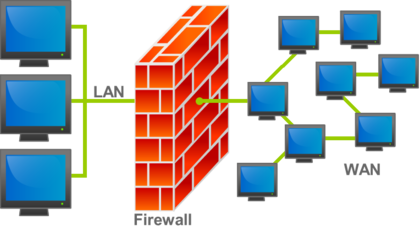
\includegraphics[scale=.7]{firewall.png}
\caption{Esquema de um firewall\footnote{\scriptsize Adaptado de
    \url{https://commons.wikimedia.org/wiki/File:Firewall.png}}.}
\end{figure}

\end{frame}

\begin{frame}{Ferramentas}

  Nos sistemas Linux o firewall normalmente utilizado é o
  \href{http://www.netfilter.org/projects/nftables/}{nftables}, e nos
  sistemas BSD, o \href{http://www.openbsd.org/faq/pf/}{pf} ({\em packet
    filter}).

\end{frame}

\begin{frame}{Regras de bloqueio}

  O firewall utiliza algumas características dos pacotes na rede,
  dentre elas:

\begin{itemize}
\item Porta de origem;
\item IP de destino;
\item Porta de destino;
\item Protocolo IP (TCP ou UDP).
\end{itemize}
\end{frame}

\begin{frame}{nftables}
\end{frame}
\begin{frame}{Cadeias}{{\it chains\/}}
\begin{tikzpicture}[node distance=2.5cm,main/.style = {draw}] 
  \node[] (ingoing) {entrada};
  \node[] (routing) [right of=ingoing] {roteamento};
  \draw[] (ingoing) -- (routing);
  \node[draw] (forward) [right of=routing] {\bf forward};
  \draw[->] (routing) -- (forward);
  \node[draw] (input) [below of=routing] {\bf input};
  \draw[->] (routing) -- (input);
  \node[draw,ellipse] (process) [below right of=input] {processos locais};
  \draw[->] (input) -- (process);
  \node[draw] (output) [above right of=process] {\bf output};
  \draw[->] (process) -- (output);  
  \node[] (outgoing) [right of=forward] {saída};
  \draw[->] (forward) -- (outgoing);
  \draw[->] (output) -- (outgoing);  
\end{tikzpicture} 
\end{frame}

 
% \date{2021-10-20}\input crypto

\end{document}
